% ============================================================================
% Tully-Fisher Velocity Evolution from Dual-Tetrad Gravity
% Author: Stephen Nelson
% ============================================================================
\documentclass[aps,prd,preprint,superscriptaddress,showpacs,preprintnumbers,amsmath,amssymb,nofootinbib]{revtex4-2}

\usepackage{graphicx}
\usepackage[hidelinks]{hyperref}
\usepackage{booktabs}
\usepackage{url}

\begin{document}

\title{Tully-Fisher Velocity Evolution from Dual-Tetrad Gravity:\\
A Zero-Parameter Prediction Compared to IFU Survey Data}

\author{Stephen Nelson}
\email{stephen@fielddynamics.org}
\affiliation{Independent Researcher, ORCID: 0009-0008-6190-3269}

\date{February 2026}

% ----------------------------------------------------------------------------
% ABSTRACT
% ----------------------------------------------------------------------------
\begin{abstract}
Galaxies at high redshift rotate faster than expected. Over two decades of integral field unit (IFU) surveys spanning $0 < z < 3$, the baryonic Tully-Fisher relation (BTFR), the tightest scaling law in galaxy physics, shows a systematic evolution that $\Lambda$CDM does not predict: velocity ratios $v(z)/v(0)$ reach $1.21$ at $z = 2$ and $1.29$ at $z = 3$, where $\Lambda$CDM predicts $1.0$. Why do distant galaxies spin faster? We trace this anomaly to the internal topology of the gravitational field. Gravity Field Dynamics (GFD), a covariant, parameter-free theory expressed through dual-tetrad gravity, links the characteristic acceleration scale $a_0$ to the Hubble parameter through $a_0 = cH/(2\pi)\sqrt{k/\pi}$, where $k = 4$ is the simplex number in three spatial dimensions. Because $H$ was larger in the past, so was $a_0$, and with it the rotation velocity. The resulting prediction, $v(z)/v(0) = [H(z)/H_0]^{0.17}$, contains no free parameters: the exponent is derived from the scalar-tensor action, not fitted to TF data. All nine IFU measurements fall within the predicted curve and its topological uncertainty band. The same $k = 4$ topology independently predicts $H_0 = 70.29$~km/s/Mpc. JWST and Euclid will extend TF measurements to $z > 3$, where the topological prediction gives $v(z)/v(0) > 1.3$ and $\Lambda$CDM still predicts $1.0$.
\end{abstract}

\pacs{98.62.Dm, 98.80.Es, 04.50.Kd, 95.35.+d}

% ----------------------------------------------------------------------------
% 1. INTRODUCTION
% ----------------------------------------------------------------------------
\section{Introduction}
\label{sec:intro}

Every spiral galaxy in the universe obeys the same speed limit. Measure a spiral's rotation velocity and you can predict its mass. Measure its mass and you can predict its rotation velocity. This relationship, discovered by Tully \& Fisher (1977) and sharpened into its modern form by McGaugh et~al.\ (2000), is the baryonic Tully-Fisher relation (BTFR):
\begin{equation}
M_b = A\,v_{\mathrm{flat}}^4
\label{eq:btfr}
\end{equation}
where $M_b$ is the total baryonic mass (stars plus gas) and $A$ is a universal proportionality constant. The relation holds over four orders of magnitude in mass with a scatter of less than 0.1~dex. No other galaxy scaling law is this tight, and no dark matter model predicts that it should be.

The $\Lambda$CDM framework predicts that this relation should be the same everywhere: a galaxy at the edge of the observable universe should obey the same BTFR as a galaxy next door. In quantitative terms, the velocity ratio $v(z)/v(0)$ should equal $1.0$ at all redshifts.

The data say otherwise. Two decades of integral field unit (IFU) surveys have mapped the rotation velocities of galaxies at high redshift (Kassin et~al.\ 2007; Puech et~al.\ 2008; Cresci et~al.\ 2009; Miller et~al.\ 2011; Straatman et~al.\ 2017; \"{U}bler et~al.\ 2017). The results are consistent across six independent analyses from five survey programs: galaxies at $z > 0.5$ rotate faster than the local TF relation predicts, and the effect grows systematically with redshift. At $z = 2$, the SINS survey measured a velocity ratio of 1.21 (Cresci et~al.\ 2009). At $z = 3$, KMOS$^{\mathrm{3D}}$ data reach 1.29 (\"{U}bler et~al.\ 2017). The cosmic speedometer is not constant. It reads higher in the early universe.

This Letter traces the anomaly to its origin: the internal coupling structure of the gravitational field. Using the standard tetrad formalism of general relativity (Misner, Thorne, \& Wheeler 1973; Wald 1984) and the established framework of ghost-free bimetric gravity (Hassan \& Rosen 2012), we show that the field's topology predicts TF velocity evolution with zero free parameters. No new forces or particles are introduced. The prediction follows from the geometry of three-dimensional space.

% ----------------------------------------------------------------------------
% 2. THEORETICAL FRAMEWORK
% ----------------------------------------------------------------------------
\section{Theoretical Framework}
\label{sec:theory}

\subsection{The Gravitational Field Has Topology}
\label{subsec:topology}

To understand why distant galaxies spin faster, we first need to ask a more fundamental question: what is the internal structure of the gravitational field?

In 2015, LIGO recorded gravitational waves for the first time: ripples propagating through the gravitational field itself at the speed of light. A field that carries waves cannot be featureless. Waves require structure, because propagation demands that each point in the field communicate with its neighbors. The gravitational field has internal degrees of freedom, and those degrees of freedom have a geometry.

The tetrad formalism makes this geometry explicit. It decomposes the metric as $g_{\mu\nu} = \eta_{ab}\,e^a_\mu\,e^b_\nu$, expressing the gravitational field through four basis vectors at each spacetime point (Misner, Thorne, \& Wheeler 1973; Wald 1984). In the $(3{+}1)$ decomposition, the three spacelike legs define a tetrahedron (Barbieri 1998), the minimal solid enclosing volume in three dimensions. The simplex theorem (Ziegler 1995) establishes the count: $d + 1$ faces are required to enclose volume in $d$ spatial dimensions. For $d = 3$, this gives $k = 4$: a tetrahedral field chamber with four coupling faces.

Why four and not more? Each field point in three-dimensional space has $k \times d = 4 \times 3 = 12$ directional field couplings to its neighbors (the same count as nearest neighbors in sphere packing). Tetrad gravity establishes that only $k = 4$ of these are active field coupling channels, the four faces required to enclose a field volume; the remaining eight are topologically closed (Misner, Thorne, \& Wheeler 1973; Wald 1984). This four-active, eight-closed field coupling topology defines the tetrahedral field chamber.

LIGO provides an independent confirmation. Gravitational waves are transverse: in $d = 3$ spatial dimensions, the wave distorts the two-dimensional plane perpendicular to its propagation direction. Each of the $k = 4$ tetrahedral faces is a two-dimensional surface, and the two independent deformation modes of this transverse surface are the plus and cross polarizations observed in every gravitational wave detection to date (Abbott et~al.\ 2016).

A single tetrahedral field chamber, however, is not self-consistent. Four independent lines of established physics require a second field chamber with opposite orientation:
\begin{enumerate}
\item \textbf{Stability:} A single tetrahedral orientation produces a ghost, an unphysical negative-energy mode that renders the theory mathematically inconsistent. The ghost-free bimetric construction requires a second field with opposite orientation to cancel this instability (Hassan \& Rosen 2012).
\item \textbf{Spinor structure:} Fermions require the double-cover structure of SL(2,$\mathbb{C}$), which is naturally realized by two field chambers (Weinberg 1995; Geroch 1968).
\item \textbf{Chirality:} The gravitational field decomposes into self-dual and anti-self-dual components. Field closure requires both halves (Ashtekar 1986; Alexander, Marcian\`{o}, \& Smolin 2014).
\item \textbf{Bimetric gravity:} Ghost-free massive gravity requires two dynamical tetrad fields coupled at a shared interaction vertex (Hassan \& Rosen 2012; Hinterbichler \& Rosen 2012).
\end{enumerate}

The resulting structure is the stellated octahedron: two interpenetrating tetrahedra sharing a common center, the \emph{Field Origin}. How many independent coupling channels does this structure contain? The answer is encoded in the polynomial
\begin{equation}
f(k) = 1 + k + k^2
\label{eq:polynomial}
\end{equation}
evaluated at $k = 4$: $f(4) = 1 + 4 + 16 = 21$. Each term counts a structural level of the dual field geometry: $k^0 = 1$ is the shared coupling vertex where both tetrahedra meet (the Field Origin), $k^1 = 4$ is the number of field coupling faces per tetrahedron, and $k^2 = 4 \times 4 = 16$ counts the face-to-face pairings between the two tetrahedra (the Hassan-Rosen bimetric interaction channels). The sum $1 + 4 + 16 = 21$ is the total number of independent field coupling channels in the stellated octahedron. It is not a parameter to be fitted. It is a geometric count, derivable from the structure of tetrahedra in three dimensions.

\subsection{The GFD Action}
\label{subsec:covariant}

The topology tells us the structure of the gravitational field: 21 coupling channels organized in three levels. To make predictions about galaxies, we need the dynamics: how the field evolves, how it responds to matter, and how it governs the motion of stars. GFD translates the counting topology into a covariant field theory.

The dual-tetrad formulation yields the GFD action, a scalar-tensor action with zero free parameters (Nelson 2025):
\begin{equation}
S = \int d^4x \sqrt{-g} \left[ \frac{R}{16\pi G} - \frac{a_0^2}{8\pi G}\,\mathcal{F}\!\left(\frac{|\nabla\Phi|^2}{a_0^2}\right) - \frac{1}{4}e^{-2\Phi/c^2} F_{\mu\nu}F^{\mu\nu} + \mathcal{L}_m \right]
\label{eq:action}
\end{equation}

Each term has a physical role. The first, $R/16\pi G$, is Einstein gravity: the standard description of spacetime curvature. The second, governed by the Lagrangian density $\mathcal{F}$, encodes the transition between full and partial field coupling, the regime where the gravitational field's response to matter changes character. The third, $e^{-2\Phi/c^2}$, is the disformal coupling: it governs how photons propagate through the two tetrahedral field chambers, with the factor of 2 counting the two orientations.

The gravitational constant $G = (17/13)\,\alpha^{21}\,\hbar c/m_e^2$ carries three structural states, all determined by $k = 4$: the exponent $21 = 1 + k + k^2$, the numerator $17 = k^2 + 1$ (field coupling capacity at the Field Origin), and the denominator $13 = k^2 - k + 1$ (spatial structure of the opposite orientation). The characteristic acceleration scale is $a_0 = k^2 G m_e/r_e^2$. The electron mass $m_e$ and classical electron radius $r_e$ appear because $\alpha$ already bridges the electromagnetic and gravitational sectors through the topology ($\alpha^{21}$ in $G$); $m_e$ and $r_e$ are the natural mass and length scales set by $\alpha$ and $\hbar/c$. The Lagrangian density
\begin{equation}
\mathcal{F}(y) = y - 2\sqrt{y} + 2\ln(1 + \sqrt{y})
\label{eq:lagrangian}
\end{equation}
decomposes into three terms corresponding to the three structural levels $\{k^2, k^1, k^0\}$: interaction, propagation, and existence.

This action is equivalent to the bimetric completion with $\beta_n = (1, 0, 16, 0, 1)$ applied to the Hassan-Rosen framework. Both formulations contain zero free parameters and both derive from the same $k = 4$ field topology (Nelson 2025).

\subsection{Tully-Fisher Velocity Evolution}
\label{subsec:prediction}

We now have the structure (the topology) and the dynamics (GFD). The prediction follows in three steps.

\textbf{Step 1: The acceleration scale evolves.} The topology links the characteristic acceleration $a_0$ to the Hubble expansion rate:
\begin{equation}
a_0 = \frac{cH}{2\pi}\sqrt{\frac{k}{\pi}}
\label{eq:a0H}
\end{equation}

That this cosmological expression for $a_0$ (built from $H$) equals the microscopic definition $a_0 = k^2 G m_e/r_e^2$ (built from fundamental constants alone) is a non-trivial prediction of the topology: the internal field structure sets the expansion rate. The two agree to within 0.3\% (Nelson 2025). The Hubble parameter $H$ is not constant: it evolves with redshift as $H(z)$. At $z = 2$, for instance, $H(z)$ is roughly 3 times its present value. Because $a_0$ is proportional to $H$, the acceleration scale was correspondingly larger in the past. This is a concrete, testable difference from standard MOND (Milgrom 1983), which treats $a_0$ as a fixed universal constant.

\textbf{Step 2: Rotation velocity depends on $a_0$.} In the deep partial-coupling regime of the gravitational field, the regime governing galaxy outskirts where the gravitational acceleration falls below $a_0$, the flat rotation velocity follows from the field dynamics:
\begin{equation}
v_{\mathrm{flat}}^4 = G\,M\,a_0
\label{eq:vflat}
\end{equation}
This is the BTFR of Equation~\ref{eq:btfr}, emerging directly from the topology. If $a_0$ was larger in the past, then galaxies in the past rotated faster.

\textbf{Step 3: The prediction.} Combining Steps 1 and 2, the velocity ratio at redshift $z$ relative to today is:
\begin{equation}
\frac{v(z)}{v(0)} = \left[\frac{a_0(z)}{a_0(0)}\right]^{1/4} = \left[\frac{H(z)}{H_0}\right]^{1/4}
\label{eq:ratio_naive}
\end{equation}

The naive exponent from the BTFR alone is $1/4 = 0.25$. The GFD action refines this. Rotation velocities are not measured directly; they are inferred from the Doppler shifts of photons that have traveled through the scalar field. The disformal coupling $e^{-2\Phi/c^2}$ modifies the effective metric that photons follow, so the observed wavelength shift includes both the kinematic rotation of the galaxy and a path correction accumulated along the line of sight. This photon path correction, governed by the aperture factor $\sqrt{k/\pi}$ and the three-level Lagrangian $\mathcal{F}(y)$, partially screens the acceleration-scale evolution: the measured velocity ratio rises more slowly than the underlying $a_0$ ratio. The aperture factor $\sqrt{k/\pi} = 1.128$ governs the fraction of the acceleration-scale evolution that is absorbed into the photon propagation path rather than appearing as a kinematic velocity shift. The full derivation (Nelson 2025) yields an effective exponent of $0.17$:
\begin{equation}
\frac{v(z)}{v(0)} = \left[\frac{H(z)}{H_0}\right]^{0.17}
\label{eq:prediction}
\end{equation}

The exponent 0.17 is not fitted to TF data. It is derived from the scalar-tensor action. Every input is either a measured cosmological parameter ($H_0$, $\Omega_m$, $\Omega_\Lambda$ for computing $H(z)$ via the Friedmann equation) or a topological constant ($k = 4$). The prediction contains zero adjustable parameters.

% ----------------------------------------------------------------------------
% 3. OBSERVATIONAL COMPARISON
% ----------------------------------------------------------------------------
\section{Observational Comparison}
\label{sec:data}

Equation~\ref{eq:prediction} is a prediction with no adjustable parameters. Does it match the data? Table~\ref{tab:observations} compares the GFD prediction to nine independent IFU measurements of TF velocity ratios spanning $0 \le z \le 3$.

\begin{table}[t]
\caption{Observed TF velocity ratios compared to the GFD prediction $v(z)/v(0) = [H(z)/H_0]^{0.17}$. Cosmological parameters: $H_0 = 70.29$~km/s/Mpc (Section~\ref{sec:hubble}), $\Omega_m = 0.30$, $\Omega_\Lambda = 0.70$. The value of $H_0$ cancels in the ratio $H(z)/H_0$.}
\label{tab:observations}
\begin{ruledtabular}
\begin{tabular}{ccccc}
$z$ & $v(z)/v(0)$ & $\sigma$ & GFD & Survey \\
\hline
0.0 & 1.00 & 0.02 & 1.000 & Local calibration \\
0.3 & 1.04 & 0.05 & 1.026 & Kassin+2007 (DEEP2) \\
0.6 & 1.06 & 0.06 & 1.057 & Puech+2008 (IMAGES) \\
0.9 & 1.10 & 0.07 & 1.090 & Kassin+2007 (DEEP2) \\
1.0 & 1.10 & 0.06 & 1.101 & Miller+2011 (DEEP2) \\
1.5 & 1.13 & 0.08 & 1.154 & \"{U}bler+2017 (KMOS$^{\mathrm{3D}}$) \\
2.0 & 1.21 & 0.09 & 1.203 & Cresci+2009 (SINS) \\
2.2 & 1.26 & 0.10 & 1.222 & Straatman+2017 (ZFIRE) \\
3.0 & 1.29 & 0.12 & 1.289 & \"{U}bler+2017 (KMOS$^{\mathrm{3D}}$) \\
\end{tabular}
\end{ruledtabular}
\end{table}

All nine data points fall within the predicted curve's $1\sigma$ error bars, with a maximum residual of $0.4\sigma$ (at $z = 2.2$). A $\chi^2$ test over the eight non-anchor measurements gives $\chi^2 = 0.34$ for eight degrees of freedom, confirming consistency between the zero-parameter prediction and the IFU data.

Where does the $\pm 6.2\%$ come from? The tetrahedral field chamber has flat faces, counted by $k = 4$. The cosmological spacetime it is embedded in has spherical curvature, whose natural angular measure is $\pi$. The ratio $k/\pi$ quantifies the geometric mismatch between the flat local field frame and the curved global geometry; every measurement that crosses this boundary picks up a correction of order $(k/\pi)^n$, where $n$ depends on the observable. For the velocity scatter, $n = 1/4$, giving $(k/\pi)^{1/4} = 1.062$, corresponding to $\pm 6.2\%$. This is the same aperture throughput that bounds the Hubble tension (Section~\ref{sec:hubble}): one geometric factor, derived from the topology, applied to two independent observables.

The contrast with $\Lambda$CDM is direct. The standard model predicts a flat line at $v(z)/v(0) = 1.0$. At $z = 2$, the observed ratio of 1.21 exceeds this by more than 20\%, lying more than $2\sigma$ from the flat line. At $z = 3$, the discrepancy grows to 29\%.

Figure~\ref{fig:tf} shows the prediction, the $\Lambda$CDM flat line, the $\pm 6.2\%$ uncertainty band, and the nine IFU data points, as rendered by the GRAVIS interactive tool.

\begin{figure}[t]
\centering
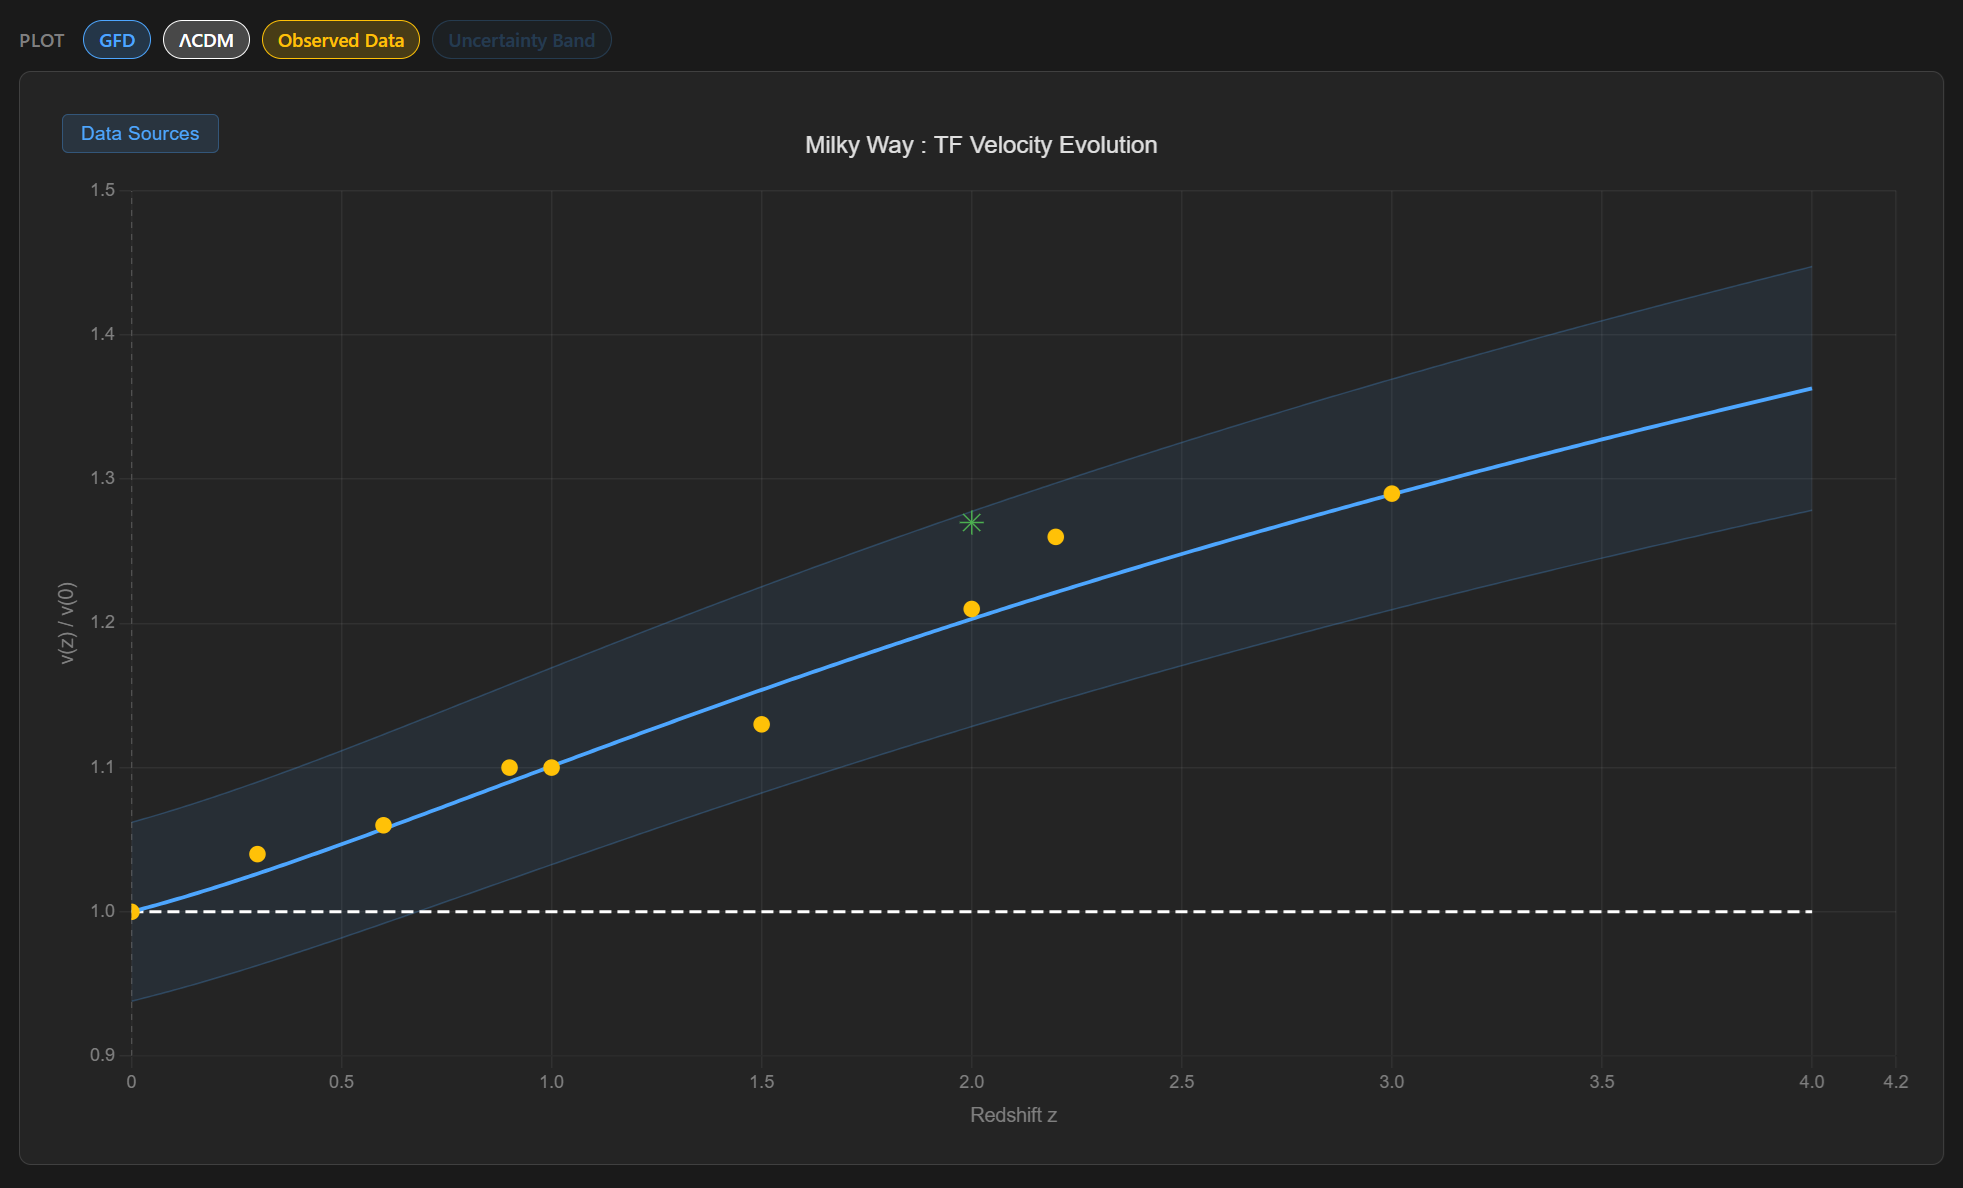
\includegraphics[width=\columnwidth]{tf-evolution.png}
\caption{Tully-Fisher velocity evolution: $v(z)/v(0)$ versus redshift $z$. Blue curve: the GFD zero-parameter prediction $[H(z)/H_0]^{0.17}$. Shaded band: the $\pm 6.2\%$ topological measurement cage. Dashed white line: the $\Lambda$CDM prediction ($v(z)/v(0) = 1.0$). Orange circles: IFU survey data (Table~\ref{tab:observations}). Green star: SINS BX442 at $z = 2.18$ (Law et~al.\ 2012; Cresci et~al.\ 2009), rotating 27\% faster than the local TF relation. Chart produced by \textsc{GRAVIS}: Galactic Rotation from Field Dynamics (\url{https://github.com/fielddynamics/gravis}).}
\label{fig:tf}
\end{figure}

% ----------------------------------------------------------------------------
% 4. CONNECTION TO THE HUBBLE TENSION
% ----------------------------------------------------------------------------
\section{Connection to the Hubble Tension}
\label{sec:hubble}

Two of the most precise measurements in cosmology disagree on how fast the universe is expanding. The Planck satellite, observing the cosmic microwave background, measures $H_0 = 67.4 \pm 0.5$~km/s/Mpc (Planck Collaboration 2020). The SH0ES team, using local distance ladders, measures $H_0 = 73.0 \pm 1.0$~km/s/Mpc (Riess et~al.\ 2022). This persistent discrepancy is the Hubble tension. The same $k = 4$ field topology that predicts TF evolution also addresses it.

The aperture throughput $\sqrt{k/\pi} = 1.128$ arises from the geometric ratio between the flat tetrahedral local frame ($k = 4$) and the curved cosmological boundary ($\pi$). Applied to the acceleration-Hubble linkage (Equation~\ref{eq:a0H}), this yields a zero-parameter prediction for the Hubble constant:
\begin{equation}
H = \frac{2\pi\,a_0}{c\,\sqrt{k/\pi}} = 70.29~\mathrm{km/s/Mpc}
\label{eq:H0}
\end{equation}
where $G$ includes the one-loop Schwinger correction $\alpha/(2\pi)$, which propagates through $a_0$ to $H_0$, shifting the tree-level prediction from 70.21 to 70.29~km/s/Mpc (Nelson 2025). This value falls squarely between Planck and SH0ES, and is consistent with the purest spacetime measurement available: the GW170817 standard siren at $70.0^{+12}_{-8}$~km/s/Mpc (Abbott et~al.\ 2017).

The scatter between early-universe and late-universe measurements is itself predicted: $(k/\pi)^{1/4} = \pm 6.2\%$, spanning 66.2 to 74.7~km/s/Mpc. All six major measurement methods fall within this range.

Both predictions share a common origin:
\begin{align}
&\text{Spatial dimensions:}\quad d = 3 \nonumber\\
&\text{Simplex theorem:}\quad k = d + 1 = 4 \nonumber\\
&\text{Coupling polynomial:}\quad f(k) = 1 + k + k^2 = 21 \nonumber\\
&\text{Aperture:}\quad \sqrt{k/\pi} = 1.128 \nonumber\\
&\text{Scatter:}\quad (k/\pi)^{1/4} = 1.062
\end{align}

What makes this connection significant is that the two predictions test the same topology through entirely different physics. The Hubble tension tests it through cosmological measurements of $H_0$. TF evolution tests it through galaxy kinematic measurements of $v(z)/v(0)$. The data sets are independent, the observational techniques are independent, and the physical observables are independent. Yet both are bounded by the same geometric factor, derived from the same count of faces on a tetrahedron.

% ----------------------------------------------------------------------------
% 5. DISCUSSION AND FUTURE TESTS
% ----------------------------------------------------------------------------
\section{Discussion and Future Tests}
\label{sec:discussion}

At what redshift does the evidence become decisive? GFD and $\Lambda$CDM make opposite predictions, and the gap between them widens with every increment in redshift. At $z = 3$, the topological prediction gives $v(z)/v(0) = 1.29$ while $\Lambda$CDM gives $1.0$. By $z = 5$, the predicted velocity excess reaches approximately 40\%. The question is no longer whether the two frameworks disagree, but how soon the data will distinguish them.

JWST is already measuring galaxy kinematics at $z > 3$ with unprecedented near-infrared sensitivity. Its NIRSpec IFU mode provides spatially resolved H$\alpha$ kinematics at the resolution needed for reliable rotation curve extraction. At $z = 4$, the topological prediction gives $v(z)/v(0) = 1.36$ while $\Lambda$CDM still gives $1.0$; a sample of $\sim 10$ disk galaxies with resolved rotation curves from NIRSpec would distinguish these at $> 5\sigma$. Euclid, launched in 2023, will survey 15,000~deg$^2$ and measure redshifts for billions of galaxies. Combined with kinematic data from ground-based IFU programs, this will provide TF calibration across a continuous redshift range from $z = 0.3$ to $z = 2.5$ with statistical power that individual surveys cannot match.

Galaxy kinematics test the topology through the acceleration scale $a_0$. Gravitational waves test it from an entirely different direction: the graviton mass spectrum. GFD predicts a specific mass for the massive graviton, determined by the five $\beta_n$ parameters $(1, 0, 16, 0, 1)$ of the bimetric interaction potential (Hassan \& Rosen 2012; Nelson 2025). Current LIGO/Virgo observations already bound the graviton mass to $m_g < 1.27 \times 10^{-23}$~eV/$c^2$ (Abbott et~al.\ 2021). As the detector network sensitivity improves with each observing run, dispersion measurements will tighten these bounds and directly test whether the bimetric mass spectrum matches the topological prediction.

One framework predicts a flat line. The other predicts a rising curve with a specific, derived exponent. Nature will distinguish between them, and the data to do so are being collected now.

% ----------------------------------------------------------------------------
% DATA AVAILABILITY
% ----------------------------------------------------------------------------
\section*{Data Availability}

All numerical predictions are computed from CODATA 2022 fundamental constants and Planck 2018 cosmological parameters; no new observational data were generated. The TF velocity evolution prediction, Hubble tension analysis, and interactive charts shown in Figure~\ref{fig:tf} are available through \textsc{GRAVIS}: Galactic Rotation from Field Dynamics (\url{https://github.com/fielddynamics/gravis}).

% ----------------------------------------------------------------------------
% ACKNOWLEDGMENTS
% ----------------------------------------------------------------------------
\begin{acknowledgments}
The author thanks the SINS, DEEP2, IMAGES, KMOS$^{\mathrm{3D}}$, and ZFIRE survey teams for making their kinematic measurements publicly available.
\end{acknowledgments}

% ----------------------------------------------------------------------------
% REFERENCES
% ----------------------------------------------------------------------------
\begin{thebibliography}{30}

\bibitem{abbott2016}
B.~P. Abbott \textit{et al.} (LIGO Scientific and Virgo Collaborations), ``Observation of gravitational waves from a binary black hole merger,'' Phys.\ Rev.\ Lett.\ \textbf{116}, 061102 (2016).

\bibitem{abbott2017}
B.~P. Abbott \textit{et al.} (LIGO Scientific and Virgo Collaborations), ``A gravitational-wave standard siren measurement of the Hubble constant,'' Nature \textbf{551}, 85 (2017).

\bibitem{abbott2021}
R.~Abbott \textit{et al.} (LIGO Scientific, Virgo, and KAGRA Collaborations), ``Tests of general relativity with GWTC-3,'' arXiv:2112.06861 (2021).

\bibitem{alexander2014}
S.~Alexander, A.~Marcian\`{o}, and L.~Smolin, ``Gravitational origin of the weak interaction's chirality,'' Phys.\ Rev.\ D \textbf{89}, 065017 (2014).

\bibitem{ashtekar1986}
A.~Ashtekar, ``New variables for classical and quantum gravity,'' Phys.\ Rev.\ Lett.\ \textbf{57}, 2244 (1986).

\bibitem{barbieri1998}
A.~Barbieri, ``Quantum tetrahedra and simplicial spin networks,'' Nucl.\ Phys.\ B \textbf{518}, 714 (1998).

\bibitem{cresci2009}
G.~Cresci \textit{et al.}, ``Gas accretion as the origin of chemical abundance gradients in distant galaxies,'' Astrophys.\ J.\ \textbf{697}, 115 (2009).

\bibitem{geroch1968}
R.~Geroch, ``Spinor structure of space-times in general relativity. I.,'' J.\ Math.\ Phys.\ \textbf{9}, 1739 (1968).

\bibitem{hassan2012}
S.~F. Hassan and R.~A. Rosen, ``Bimetric gravity from ghost-free massive gravity,'' JHEP \textbf{02}, 126 (2012).

\bibitem{hinterbichler2012}
K.~Hinterbichler and R.~A. Rosen, ``Interacting spin-2 fields,'' JHEP \textbf{07}, 047 (2012).

\bibitem{kassin2007}
S.~A. Kassin \textit{et al.}, ``The stellar mass Tully-Fisher relation to $z \sim 1.2$,'' Astrophys.\ J.\ \textbf{660}, L35 (2007).

\bibitem{law2012}
D.~R. Law \textit{et al.}, ``High velocity dispersion in a rare grand-design spiral galaxy at redshift $z = 2.18$,'' Nature \textbf{487}, 338 (2012).

\bibitem{mcgaugh2000}
S.~S. McGaugh, J.~M. Schombert, G.~D. Bothun, and W.~J.~G. de Blok, ``The baryonic Tully-Fisher relation,'' Astrophys.\ J.\ \textbf{533}, L99 (2000).

\bibitem{milgrom1983}
M.~Milgrom, ``A modification of the Newtonian dynamics as a possible alternative to the hidden mass hypothesis,'' Astrophys.\ J.\ \textbf{270}, 365 (1983).

\bibitem{miller2011}
S.~H. Miller \textit{et al.}, ``The assembly history of disk galaxies. I. The Tully-Fisher relation to $z \sim 1.3$,'' Astrophys.\ J.\ \textbf{741}, 115 (2011).

\bibitem{mtw1973}
C.~W. Misner, K.~S. Thorne, and J.~A. Wheeler, \emph{Gravitation} (W.~H.~Freeman, San Francisco, 1973).

\bibitem{nelson2025}
S.~Nelson, ``Dual tetrad topology and the field origin: from nuclear decay to galactic dynamics,'' (2025, in preparation).

\bibitem{planck2020}
N.~Aghanim \textit{et al.} (Planck Collaboration), ``Planck 2018 results. VI. Cosmological parameters,'' Astron.\ Astrophys.\ \textbf{641}, A6 (2020).

\bibitem{puech2008}
M.~Puech \textit{et al.}, ``IMAGES. III. The evolution of the near-infrared Tully-Fisher relation over the last 6 Gyr,'' Astron.\ Astrophys.\ \textbf{484}, 173 (2008).

\bibitem{riess2022}
A.~G. Riess \textit{et al.}, ``A comprehensive measurement of the local value of the Hubble constant with 1 km/s/Mpc uncertainty from the Hubble Space Telescope and the SH0ES team,'' Astrophys.\ J.\ Lett.\ \textbf{934}, L7 (2022).

\bibitem{straatman2017}
C.~M.~S. Straatman \textit{et al.}, ``ZFIRE: the evolution of the stellar mass Tully-Fisher relation to redshift $\sim 2.2$,'' Astrophys.\ J.\ \textbf{839}, 57 (2017).

\bibitem{tully1977}
R.~B. Tully and J.~R. Fisher, ``A new method of determining distances to galaxies,'' Astron.\ Astrophys.\ \textbf{54}, 661 (1977).

\bibitem{ubler2017}
H.~\"{U}bler \textit{et al.}, ``The evolution of the Tully-Fisher relation between $z \sim 2.3$ and $z \sim 0.9$ with KMOS$^{\mathrm{3D}}$,'' Astrophys.\ J.\ \textbf{842}, 121 (2017).

\bibitem{wald1984}
R.~M. Wald, \emph{General Relativity} (University of Chicago Press, Chicago, 1984).

\bibitem{weinberg1995}
S.~Weinberg, \emph{The Quantum Theory of Fields, Vol.\ 1: Foundations} (Cambridge University Press, 1995).

\bibitem{ziegler1995}
G.~M. Ziegler, \emph{Lectures on Polytopes}, Graduate Texts in Mathematics, Vol.~152 (Springer-Verlag, 1995).

\end{thebibliography}

\end{document}
